\chapter{\texorpdfstring{$\Lambda_b^0$}{Lambdab} and \texorpdfstring{$\Lambda^0$}{Lambda} decay vertex reconstruction}
\label{cap:vertex_reconstruction}
This chapter details my work towards the improvement of the vertex reconstruction process for decays involving T tracks.
Section \ref{sec:reco_algorithms} delves into a deep study of the vertexing process at LHCb and the two algorithms employed in this thesis;
Section \ref{sec:reco_efficiency} introduces the problem of low vertexing efficiency for the decay of interest $\Lambda_b^0 \rightarrow J/\psi~\Lambda^0$;
Section \ref{sec:characterization_non_converged} presents my efforts in the characterization of the non-converged events in search for the root cause of the vertexing falure;
finally, Section \ref{sec:recovery_general} proposes my solution to improve the signal yield through partial recovery of non-reconstructed events.

\section{Vertex reconstruction algorithms at LHCb}
\label{sec:reco_algorithms}

\subsection{Vertex Fitter algorithm}
The Vertex Fitter (VF), implemented as part of the LoKi analysis toolkit, is the main vertexing algorithm used for the reconstruction of the $\Lambda_b^0$ decay.

Under VF formalism, each daughter particle is represented by a 7-dimensional vector\footnote{This chapter assumes the standard right-handed LHCb coordinate system, see Section \ref{info:LHCb_system}.}
\begin{equation}
	\vec{p} = \begin{pmatrix}
		\vec{r} \\ \vec{q}
	\end{pmatrix}
	=
	\begin{pmatrix}
		r_x \\ r_y \\ r_z \\ p_x \\ p_y \\ p_z \\ E
	\end{pmatrix},
	\label{eq:particle_representation}
\end{equation}
containing its 4-momentum $\vec{q}$ computed at the \textit{reference point} $\vec{r}$.
This parameter vector has an associated covariance matrix $V$, which can be written in block structure as
\begin{equation}
	\begin{pmatrix}
		V_r      & V_{rq} \\
		V_{rq}^T & V_q
	\end{pmatrix}.
	\label{eq:par_covmatrix}
\end{equation}
It is also convenient to identify its formal inverse matrix $G := V^{-1}$, which has an analogous block form:
\begin{equation}
	\begin{pmatrix}
		G_r      & G_{rq} \\
		G_{rq}^T & G_q
	\end{pmatrix}
	=
	\begin{pmatrix}
		V_r      & V_{rq} \\
		V_{rq}^T & V_q
	\end{pmatrix}^{-1}
\end{equation}

Taking the daughter particles as inputs, the Vertex Fitter will output the best fit value $\vec{x}$ for the common origin vertex, along with its covariance matrix $C$ and the $\chi^2$ to evaluate the goodness of fit.

The algorithm builds the decay tree from the bottom-up via a <<leaf-by-leaf>> approach, fitting one vertex at a time (e.g. $J/\psi \rightarrow \mu^+ \mu^-$, $\Lambda^0 \rightarrow p \pi^-$) and then moving upwards (e.g. $\Lambda_b^0 \rightarrow J/\psi~\Lambda^0$).
This process is blind to the downstream leaves and only considers kinematic information of the immediate daughter particles, without accounting for momenta and mass constraints.

\subsubsection{Iterating paradigm}
The basic unit of recursion of the Vertex Fitter is the \textit{iteration}:
the algorithm is set to repeat the vertexing process until either a convergence condition is satisfied (see later) or the fit reaches the set number of allowed iterations, 10 by default.
In the latter case, a non-convergence error is thrown and the candidate event is discarded.

At the beginning of each iteration, the final vertex covariance matrix $C^{i-1}_n$ from the previous iteration\footnote{The subscript $n$ identifies the final step number, see later.} is scaled down by a factor $s^2 = {10}^{-4}$:
\begin{equation}
	C^{i}_0 = C^{i-1}_n \times s^2.
\end{equation}
The algorithm then performs a \textit{proper transportation}, a dedicated routine in which all daughter particles are extrapolated to the $z$ component of the current (tentative) position of the common production vertex $\vec{x}_n^{i-1}$.
%Such transportation is also performed at the end of the vertexing procedure to ensure an optimal computation of final particle momenta.

Extrapolation using T tracks is a sensitive affair:
unlike the case for other track types, no constraints are available besides the downstream measurement performed by the T tracking stations, meaning the tracks have to be propagated through several meters while accounting for the intense and non-homogeneous LHCb magnetic field.
For this analysis, said extrapolation was performed via numerical solution of the track propagation equations using an approach based on the Runge-Kutta method \cite{Bos:1070314} \cite{Hairer1993}.

%---
%
%When all particles have been added, i.e. all steps have been performed, the algorithm concludes an \textit{iteration}.
%The process is then repeated 
%
%Within an individual iteration, the vertex position is updated at each step following \eqref{eq:VF_new_vertex_final}.
%Consequently, the individual momenta of the particles must also be updated to reflect the change in reference point;
%this is performed with a degree of approximation in equation \eqref{eq:VF_new_momentum_final}.
%To supplement this, every iteration begins with a \textit{proper transportation}

%\subsubsection{Old}
%
%combining the position $\vec{x}$ of the estimated origin vertex of the track (known as \textit{reference point}) with the  of the track constrained to originate in $\vec{x}$.
%At the end of the fitting process,  will coincide with the common vertex chosen for all daughter particles.
%
%In the VF framework it's sometimes useful to write vector particle vector $\vec{p}_k$ in terms of $\vec{x}_k$ and $\vec{q}_k$ via a projection matrix formalism:
%\begin{equation}
%	\vec{p}_k = c^0_k + A_k \vec{x}_k + B_k \vec{q}_k,
%\end{equation}
%with $A_k$ and $B_k$ defined as
%\begin{equation}
%A_k = \left[
%	\frac{\partial \vec{p}_k}{\partial \vec{x}_k}
%\right],
%\quad\quad 
%B_k = \left[
%	\frac{\partial \vec{p}_k}{\partial \vec{q}_k}
%\right].
%\end{equation}
%Of course, the simple representation described in \eqref{eq:particle_representation} allows for likewise simple projection matrices:
%\begin{equation}
%A_k = A = \begin{pmatrix}
%1 \\
%0
%\end{pmatrix},
%\quad\quad 
%B_k = B = \begin{pmatrix}
%0 \\
%1
%\end{pmatrix}.
%\end{equation}
%
%--

\subsubsection{Step}
Within an individual iteration $i$, denoted by a superscript, the Vertex Fitter algorithm proceeds by \textit{steps} denoted by subscripts, with each step $k$ coinciding with the addition of the $k$-th daughter particle.

Given information on the vertex position $\vec{x}_{k-1}$ obtained using the first $k-1$ particles, track $k$ is added through the following recursive procedure.
First the inverse vertex covariance matrix is updated:
\begin{equation}
C_k^{-1} = C_{k-1}^{-1} + {V_r}_k^{-1},
\end{equation}
where the reference point inverse covariance matrix ${V_r}_k^{-1}$ has been updated at the beginning of the iteration through the proper transportation phase.

%\begin{equation}
%G_k^B = G_k - G_k B_k W_k B_k^T G_k.
%\end{equation}
%The above auxiliary matrix depends from the particle parameter inverse covariance matrix $G_k$, extrapolated at the current vertex position (see the next paragraph), as well as from the matrix
%and
%\begin{equation}
%W_k = {\left(B_k^T G_k B_k\right)}^{-1}.
%\end{equation}

%After this, $C_k^{-1}$ is inverted and the algorithm updates the correlation matrix $E_k \coloneqq \text{corr}(\vec{x}_{k},\vec{q}_k)$ between vertex position and $k$-th particle momentum
%\begin{equation}
%E_k = -F_k C_k
%\end{equation}
%and the momentum covariance matrix
%\begin{equation}
%D_k = W_k - E_k F_k^T,
%\end{equation}
%with
%\begin{equation}
%F_k = W_k B_k^T G_k A_k.
%\end{equation}

If $C_k^{-1}$ can successfully be inverted, the algorithm updates the current best estimate of the common origin vertex:

\begin{equation}
\vec{x}_k = C_k \left[
	C_{k-1}^{-1} \vec{x}_{k-1}
	+ {V_r}_k^{-1} \vec{r}_k
\right].
\label{eq:VF_new_vertex_final}
\end{equation}

To conclude the step, the vertex $\chi^2$ is updated to the account for the new position:
\begin{equation}
\begin{aligned}
	\chi^2_k &= \chi^2_{k-1} \\
	&+
	{\left(\vec{r}_{k} - \vec{x}_k\right)}^T  {V_r}_k^{-1} \left(\vec{r}_{k} - \vec{x}_k \right) \\
	&+
	{\left(\vec{x}_k - \vec{x}_{k-1}\right)}^T  C_{k-1}^{-1} \left(\vec{x}_k - \vec{x}_{k-1}\right) \\
\end{aligned}.
\label{eq:VF_vertex_chi2_final}
\end{equation}

%Finally the step concludes with the computation of a new estimated vertex position
%\begin{equation}
%\vec{x}_k = C_k \left[
%	C_{k-1}^{-1} \vec{x}_{k-1}
%	+
%	A_k^T G_k^B \left(
%		\vec{p_k} - c_k^0	
%	\right)
%\right],
%\end{equation}
%a new 4-momentum for the $k$-th track
%\begin{equation}
%\vec{q}_k = W_k B_k^T G_k \left[
%	\vec{p_k} - c_k^0 - A_k \vec{x}_k
%\right],
%\end{equation}
%and an updated $\chi^2$ to evaluate the goodness of the best fit value for the decay vertex
%\begin{equation}
%\begin{aligned}
%\chi^2_k &= \chi^2_{k-1} \\
%&+
%\left[
%	\vec{p} - c_k^0 - A_k \vec{x}_k - B_k\vec{q}_k
%\right]^T G_k \left[
%	\vec{p} - c_k^0 - A_k \vec{x}_k - B_k\vec{q}_k
%\right] \\
%&+
%\left[
%	\vec{x}_k - \vec{x}_{k-1}
%\right] C_{k-1}^{-1} \left[
%	\vec{x}_k - \vec{x}_{k-1}
%\right]
%\end{aligned}.
%\end{equation}

%So far...
%
%\begin{equation}
%G_k = \begin{pmatrix}
%G_x 		&& G_{xp} \\
%G^T_{xp} 	&& G_p
%\end{pmatrix}
%\end{equation}
%
%\begin{equation}
%W_k = G_p^{-1}
%\end{equation}
%
%\begin{equation}
%G_k^B = \begin{pmatrix}
%G_x - G_{xp}G_p^{-1}G_{xp}^T 	&& 0 \\
%0								&& 0
%\end{pmatrix}
%\end{equation}
%
%\begin{equation}
%F_k = G_p^{-1} G_{xp}^T
%\end{equation}
%
%\begin{equation}
%C_k^{-1} = C_{k-1}^{-1} + \left[
%	G_x - G_{xp}G_p^{-1}G_{xp}^T
%\right]
%\end{equation}
%
%\begin{equation}
%E_k = -G_p^{-1} G_{xp}^T C_k
%\end{equation}
%
%\begin{equation}
%D_k = G_p^{-1} + G_p^{-1} G_{xp}^T C_k G_{xp} G_p^{-1}
%\end{equation}
%
%
%
%\begin{equation}
%\vec{q}_k = \begin{pmatrix}
%	G_p^{-1} G_{xp}^T && 0
%\end{pmatrix}
%\left[
%	\vec{p_k} - c_k^0 - A\vec{x}_k
%\right]
%\label{eq:VF_new_momentum_final}
%\end{equation}
%
%\begin{equation}
%\begin{pmatrix}
%	G_x && G_{xp} \\
%	G_{xp}^T && G_p
%\end{pmatrix}
%=
%\begin{pmatrix}
%	V_x && V_{xp} \\
%	V_{xp}^T && V_p
%\end{pmatrix}^{-1}
%\end{equation}
%
%\begin{subequations}
%\begin{align}
%&G_x - G_{xp} G_p^{-1} G_{xp} 	= V_x^{-1} \\
%&G_p^{-1} 						= V_p - V_{xp}^T V_x^{-1} V_{xp} \\
%&G_p^{-1} G_{xp}^T 				= -V_{xp}^T V_x^{-1}
%\end{align}
%\end{subequations}

\subsubsection{Seeding}

As one can observe, the procedure described above requires, at each step, both a previous estimated vertex position $\vec{x}_{k-1}$ and an associated inverse covariance matrix $C_{k-1}^{-1}$. In particular, step $k=1$ demands the existence of $\vec{x}_0$ and $C_{0}^{-1}$.

For iterations $i>1$, such roles are handily filled by the final vertex computed during the previous iteration.
For the purpose of providing the first step of the first iteration with these values, at the beginning the algorithm tries to extract a \textit{vertex seed}, a first estimate of the decay vertex position, through a dedicated procedure depending on decay topology and properties of particles involved.

In the case of interest of the $\Lambda^0 \rightarrow p \pi^-$ two-body decay, said procedure is a simplified step of the Kalman filter:
\begin{subequations}
\begin{align}
	&C^{-1}_0 = {V_r}_1^{-1}  + {V_r}_2^{-1} \\
	&\vec{x}_0 = C_0 \left(
		{V_r}_1^{-1} \vec{r}_1 + {V_r}_2^{-1} \vec{r}_2
	\right)
\end{align}
\end{subequations}
Subscripts $1$ and $2$ as used above refer to the two daughter particles in the decay (i.e. proton and pion).

\subsubsection{Termination and smoothing}
The two VF convergence conditions are both based on comparisons between the vertex position computed at the end of the current iteration with the one from the previous iteration, with convergence being called if either one of them is satisfied.

The first condition is placed on the absolute distance between the vertices:
\begin{equation}
	\left\|
	\vec{x}_n^{i} - \vec{x}_n^{i-1}
	\right\| \leq d_1
	\label{eq:cond_conv_1}
\end{equation}
where $d_1 = \SI{1}{\micro\meter}$ by default.
The second condition, by far the more commonly satisfied one when reaching convergence, is a condition on vertex distance <<in $\chi^2$ units>>:
\begin{equation}
	{\left(
	\vec{x}_n^{i} - \vec{x}_n^{i-1}
	\right)}^T
	{C_n^i}^{-1}
	\left(
	\vec{x}_n^{i} - \vec{x}_n^{i-1}
	\right)
	\leq d_2
	\label{eq:cond_conv_2}
\end{equation}
with $d_2 = 0.01$.
While condition \eqref{eq:cond_conv_1} can be satisfied at any point in the vertexing process, \eqref{eq:cond_conv_2} convergence additionally requires $i>1$, thereby excluding the very first iteration.

When convergence is reached, the algorithm applies a smoothing process: for each daughter particle, the reference point $\vec{x}_k$ is fixed to the final vertex position $\vec{x}_n^{i}$ and the momentum $\vec{q}_k$ is updated accordingly as

\begin{equation}
	\vec{q}_k =
	\vec{q}_n^i
	-
	{V_{rq}}_k
	{V_r}_k^{-1}
	\left(
		\vec{r}_k - \vec{x}_k
	\right)
\end{equation}

Finally comes the evaluation of the relevant covariance matrices. The vertex covariance matrix $C$ is obviously fixed at $C_n^i$; the algorithm also computes for each entry the correlation matrix $E_k \coloneqq \text{corr}\left(\vec{x},\vec{q}_k\right)$ between the vertex position and the particle momentum
\begin{equation}
	E_k = - F_k C,
	\label{eq:Ek}
\end{equation}
and the particle momentum covariance matrix
\begin{equation}
	D_k =
	{V_q}_k
	-
	{V_{rq}}_k {V_r}_k^{-1} {V_{rq}}_k^T
	+
	F_k C F_k^{-1},
	\label{eq:Dk}
\end{equation}
with
\begin{equation}
	F_k =
	- {V_{rq}}_k {V_r}_k^{-1}
	\label{eq:Fk}
\end{equation}
being an auxiliary matrix.

\subsubsection{Mother particle creation}
Assuming the found vertex is inside the LHCb fiducial volume, the fit is validated and a $\chi^2$ is determined by taking the last step value from \eqref{eq:VF_vertex_chi2_final} and adding the $\chi^2$ from any short-lived daughter particle.
Degrees of freedom (DOFs) for $\chi^2$ reduction are computed as follows:
\begin{itemize}
	\item each track contributes 2 DOFs;
	\item each $\rho^+$-like particle\footnote{A $\rho^+$-like particle is a particle resulting from the combination of 1 long-lived particle and $\geq 2$ photons. The category identifier is owed to the topology of the $\rho^+ \rightarrow \pi^+\pi^0$ decay with $\pi^0 \rightarrow \gamma \gamma$.} contributes 2 DOFs;
	\item each sub-vertex contributes 3 DOFs plus further DOFs from the downstream decay tree;
	\item the sum total is reduced by 3. %% Perché?
\end{itemize}

A mother particle is subsequently created using the \eqref{eq:particle_representation} representation with reference point $\vec{x}_\text{mother}$ fixed to the new-found vertex coordinates.
Its 4-momentum is computed as a simple sum of the 4-momenta of its daughters extrapolated at the vertex:
\begin{equation}
	\vec{q}_\text{mother} = \sum_{k \in \text{daughters}} \vec{q}_k.
\end{equation}

The parameter vector covariance matrix \eqref{eq:par_covmatrix} is determined as follows:
\begin{equation}
	V_{r}^\text{mother} = C,
\end{equation}
\begin{equation}
	V_{q}^\text{mother} = \sum_{k \in \text{daughters}} \left[
		D_k
		+
		\sum_{\substack{j\in\text{daughters} \\ j \neq k}}
		\left(
			F_k C F_j^T + F_j C F_k^T
		\right)
	\right],
\end{equation}
\begin{equation}
	V_{rq}^\text{mother} = \sum_{k \in \text{daughters}} E_k,
\end{equation}
with $D_k$, $E_k$ and $F_k$ for each daughter resulting from \eqref{eq:Dk}, \eqref{eq:Ek} and \eqref{eq:Fk} respectively.

Finally, the mother particle measured mass $M_\text{mother}$ is computed as magnitude of 4-vector $\vec{q}_\text{mother}$ in the $(-,-,-,+)$ metric
\begin{equation}
	M_\text{mother} = \sqrt{E_\text{mother}^2
	- {p_x}_\text{mother}^2
	- {p_y}_\text{mother}^2
	- {p_z}_\text{mother}^2
	},
\end{equation}
Its associated uncertainty is defined as
\begin{equation}
	\sigma_M^\text{mother} = \sqrt{
		\frac{1}{4 M_\text{mother}^2}
		v^T
		H
		v
	},
\end{equation}
with
\begin{equation}
	v \coloneqq \frac{dM_\text{mother}^2}{d\vec{q}}
	= \begin{pmatrix}
		-2 {p_x}_\text{mother} \\
		-2 {p_y}_\text{mother} \\
		-2 {p_z}_\text{mother} \\
		2 E_\text{mother}
	\end{pmatrix}
\end{equation}
and
\begin{equation}
	H \coloneqq \sum_{k \in \text{daughters}} {V_q}_k.
\end{equation}

\subsection{Decay Tree Fitter algorithm}
While the leaf-by-leaf approach adopted by the Vertex Fitter is fast, it brings alongside it the significant drawback of forgoing upstream information when fitting the downstream branches of a decay.
This is especially notable for decays like $K_S^0 \rightarrow \pi^0\pi^0 \rightarrow \gamma\gamma\gamma\gamma$, where the final state has no tracks to form a vertex with.
Even in the relatively more traditional case of the $\Lambda_b^0 \rightarrow J/\psi~\Lambda^0$ decay, however, the VF algorithm still limits our options.
In particular, it prevents the placing of \textit{mass constraints} on mother particles, where the fit fixes the invariant mass of the $p\pi^-$ pair to the PDG value for $m(\Lambda^0)$, for instance.

To combat this problem, all reconstructed events in this analysis undergo a refit process based on the Decay Tree Fitter (DTF) algorithm \cite{Hulsbergen:2005pu} first developed in BaBar.
This algorithm takes the entire decay chain as input and allows to place mass constraints on $p\pi^-$ and $\mu^+\mu^-$ invariant masses to match $m(\Lambda^0)$ and $m(J/\psi)$ respectively.

%% @todo: Ci starebbe un bel test in cui confronti la distribuzione dei vertici VF e DTF per mostrare che sono uguali (lo sono, vero??). Devi estrarli via Kinematic, immagino, perché nel rootfile non ci sono.

\begin{figure}[t]
	\centering
	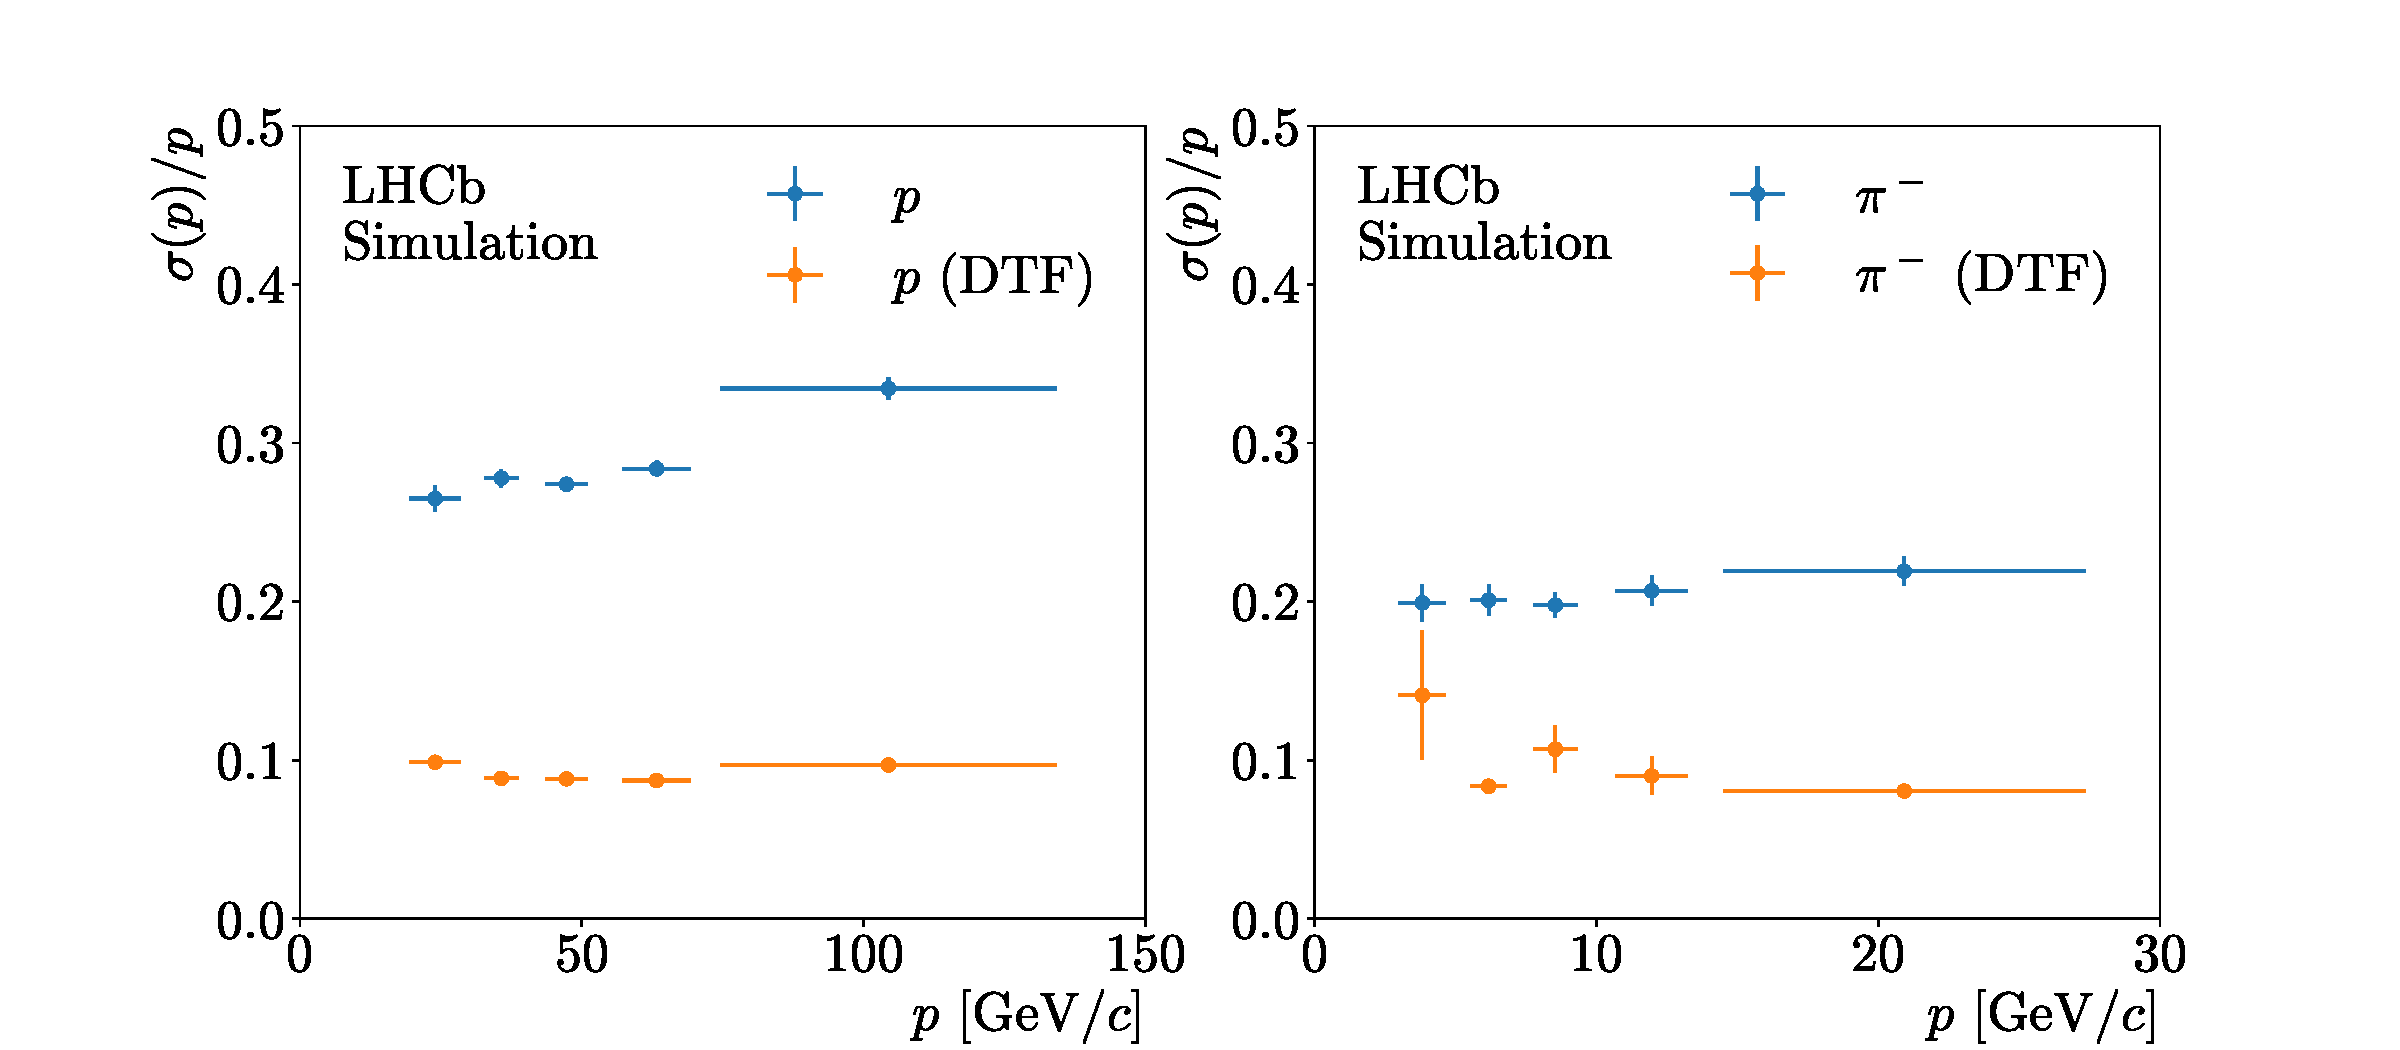
\includegraphics[width=\textwidth]{graphics/04-event_selection/paper_momentum_resolutions.pdf}
	\caption[Momentum resolution.]{Momentum resolution.}
	\label{fig:paper_momentum_resolutions}
\end{figure}

While this step introduces another filtering process and related efficiency to account for\footnote{DTF convergence efficiency with the double mass constraint is relatively uneven across the $z_\Lambda^\textbf{vtx}$ spectrum, starting at $\approx 50\%$ for $z_\Lambda^\textbf{vtx} \approx \SI{6}{\meter}$ and growing up to $\approx 85\%$ for $z_\Lambda^\textbf{vtx} \approx \SI{7.5}{\meter}$.
Comparably, vertex reconstruction is still the primary cause of event loss in this analysis.}, it proves invaluable for our physics motivations as it mitigates the most problematic drawback of T track usage, momentum resolution.
As shown in Figure \ref{fig:paper_momentum_resolutions}, using both $J/\psi$ and $\Lambda^0$ mass constraints improves $\vec{p}$ resolution from $20 \div 30\%$\footnote{Pion momentum resolution is higher because the pion receives a smaller fraction of the $\Lambda^0$ momentum, thereby having a larger bending curve than the proton and allowing for better momentum measurement at the T stations.} to $\approx 10\%$.

%% Con KineAtVtx non è più vero.
%For the purposes of the helicity angle analysis outlined in Section \ref{sec:lambda}, particle momenta computed with the DTF algorithm are particularly valuable because, in addition to their greater accuracy, they are provided directly at the production vertex;
%by contrast, VF momenta are provided either at the decay vertex (short-lived particles) or at the position of first measurement (long-lived or stable particles).

\section{Reconstruction efficiency of the \texorpdfstring{$\Lambda^0_b$}{Lambdab} and \texorpdfstring{$\Lambda^0$}{Lambda} decays}
\label{sec:reco_efficiency}

To compute the vertex reconstruction efficiency for the $\Lambda_b^0$ decay chain, it is useful to conceptualize our event selection as a five step process:
\begin{enumerate}
	\item reconstruction of associated tracks for all charged daughter particles;
	\item reconstruction of the three decay vertices ($\Lambda^0$, $J/\psi$ and $\Lambda_b^0$);
	\item preliminary selections based on kinematic variables to filter out most background (see Section \ref{sec:prefilter});
	\item Decay Tree Fitter refit with appropriate mass constraints for the analysis at hand (usually $J/\psi$ and $\Lambda^0$);
	\item further selections applied to events passing all previous steps. Detailed in Chapter \ref{cap:event_selection}, these include a physical background veto and signal selection via a trained multivariate classifier.
\end{enumerate}

For the purposes of this section, we are interested in the first two steps (track and vertex reconstruction).

Efficiencies are computed with respect to \textit{reconstructible} particles, a flag attributed during the simulation process based on the number of \textit{hits} (charged clusters with defined positions) in specific modules of the LHCb detector.
A track is said to be reconstructible as VELO track with hits in $\geq 3$ VELO modules, while it's reconstructible as T track with $\geq 1$ hits in both the $x$ and stereo layers of each T station.
If these conditions are satisfied simultaneously, the track qualifies for reconstructibility as Long track \cite{Li:2752971}.

At Monte Carlo level, a track is deemed to be \textit{reconstructed} if it can be successfully matched to at least one MC particle;
for T and Long tracks, this is true if at least $70\%$ of the hits from the respective relevant detectors for reconstructibility are shared between reconstructed and true track. For $\Lambda^0_b$ events with a true $z_\text{vtx}^\Lambda \in [\SI{6.0}{\meter}, \SI{7.6}{\meter}]$, this results in a track reconstruction efficiency in the 60\% to 80\% range.

\begin{figure}[t!]
	\centering
	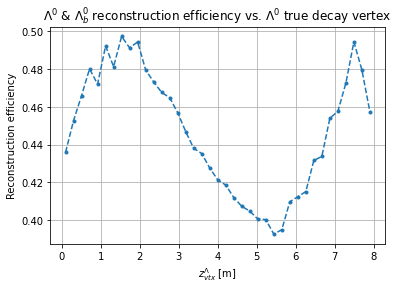
\includegraphics[width=.6\textwidth]{graphics/03-vertex_reconstruction/lambda_lambdab_reco_efficiency.png}
	\caption[A]{Reconstruction efficiency of simulated $\Lambda^0_b \rightarrow J/\psi~(\rightarrow \mu^+\mu^-)~\Lambda^0~(\rightarrow p\pi^-)$ events as function of the $z$ component of the true $\Lambda^0$ decay vertex. Assuming a $\approx 100\%$ reconstruction rate for the $J/\psi$ decay, the low efficiency is attributed to failure in reconstructing $\Lambda^0$ and $\Lambda^0_b$ decay vertices.}
	\label{fig:lambda_lambdab_reco_efficiency}
\end{figure}

When considering how many of these reconstructed charged particles pass the vertex reconstruction (\textit{vertexing}) process, the computed efficiency is much lower.
Figure \ref{fig:lambda_lambdab_reco_efficiency} plots the resulting $\Lambda_b^0$ vertexing efficiency through the whole true $z_\text{vtx}^\Lambda$ spectrum, showing that said efficiency never manages to get past the 50\% threshold.
This means that over half of our candidate signal events is lost during the second step of the five step selection process.

While available information does not distinguish between the three individual vertexing phases ($J/\psi$, $\Lambda^0$ and $\Lambda_b^0$), we can make some reasonable assumptions.
Being Long tracks, muons and antimuons have well reconstructed momentum with constraints across the LHCb detector;
for this reason their influence on the vertexing efficiency dip is considered negligible.
Furthermore, the rare usage of T tracks for physics analysis in LHCb suggests that problems are likelier to arise in the $\Lambda^0 \rightarrow p\pi^-$ vertexing and then cascade into the $\Lambda_b^0 \rightarrow J/\psi~\Lambda^0$ reconstruction.

For the above reasons, in the following sections I'll focus on the $\Lambda^0 \rightarrow p\pi^-$ decay to search for issues and solutions, with the goal of improving signal yield.


\section{Characterization of non-converged events}
\label{sec:characterization_non_converged}

\subsection{Behaviour through VF iterations}
\label{sec:oscillation}
The VF process reaches convergence if either condition \eqref{eq:cond_conv_1} or \eqref{eq:cond_conv_2} is satisfied, i.e. if the vertex position estimated at iteration $i$ and the one from iteration $i-1$ are <<close enough>> either in absolute distance or $\chi^2$ distance, up until $i_\text{max} = 10$.
This is predicated on the principle that the algorithm refines its vertex estimate after each iteration, homing in on the candidate vertex with the lowest $\tilde{\chi}^2_\text{vtx}$.

Such a behaviour is not found in non-converging (henceforth also known as \textit{failed}) events.
This can be seen by increasing $i_\text{max}=100$, which causes a negligible $\approx 2\%$ increase in converged events.
It follows that, for the vast majority of missing events, failure of convergence is not a product of low computation time and must instead result from some internal malfunction of the vertexing process.

\begin{figure}[t]
	\centering
	\begin{subfigure}{.45\textwidth}
		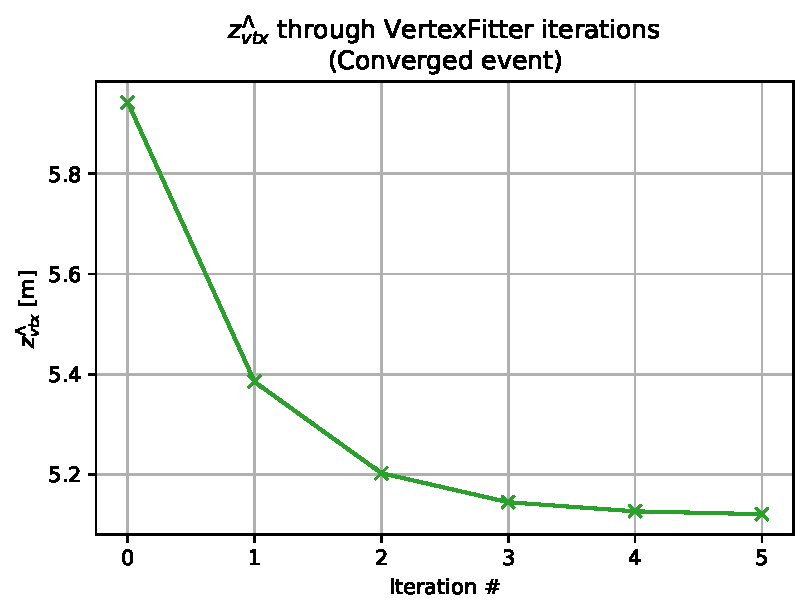
\includegraphics[width=\textwidth]{graphics/03-vertex_reconstruction/evt_converged_z_iter.pdf}
		\caption{}
		\label{fig:z_iter_conv}
	\end{subfigure}
	\begin{subfigure}{.45\textwidth}
		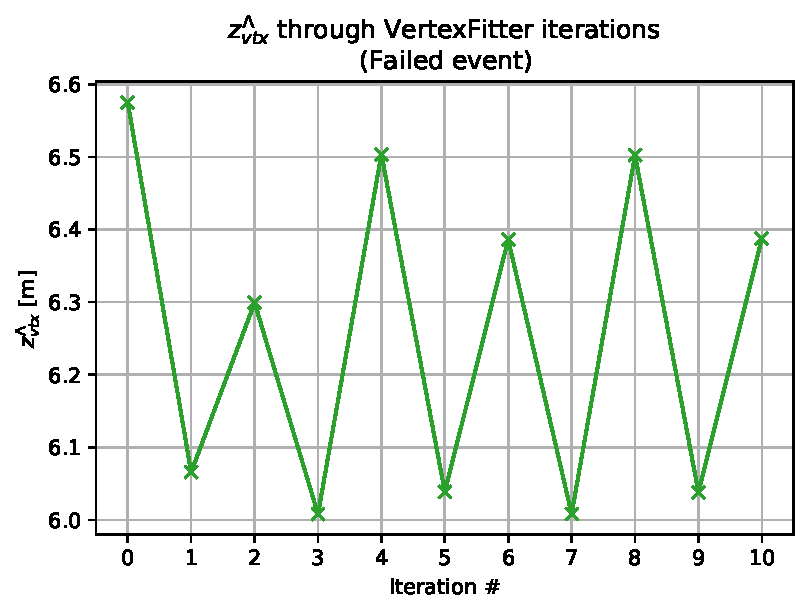
\includegraphics[width=\textwidth]{graphics/03-vertex_reconstruction/evt_failed_z_iter.pdf}
		\caption{}
		\label{fig:z_iter_failed}
	\end{subfigure}
	\caption[A and b.]{Left right}
	\label{fig:z_iter_conv_vs_failed}
\end{figure}

This is readily apparent when studying the vertex positions throughout the iterating process for examples of converged and failed events of simulated signal.
Figure \ref{fig:z_iter_conv_vs_failed} compares the values of $z_\Lambda^\text{vtx}$, the $z$ component of the $\Lambda^0 \rightarrow p\pi^-$ decay vertex, as reconstructed by the VF in iterations $0$ to $10$ ($i=0$ being the starting seed).
Figure \ref{fig:z_iter_conv} (converged) exhibits the expected behaviour, with the algorithm refining its vertex estimate after every iteration and finally converging as early as $i=5$.
By contrast, \ref{fig:z_iter_failed} (failed) presents an \textit{oscillating behaviour} of $z_\Lambda^\text{vtx}$, constantly flipping the probing direction after an iteration completes.
While a particularly tricky instance of the first type of event may potentially benefit by an increased $i_\text{max}$, no amount of allotted computations can lead the second type to convergence.

\begin{figure}[t]
	\centering
	\begin{subfigure}{.45\textwidth}
		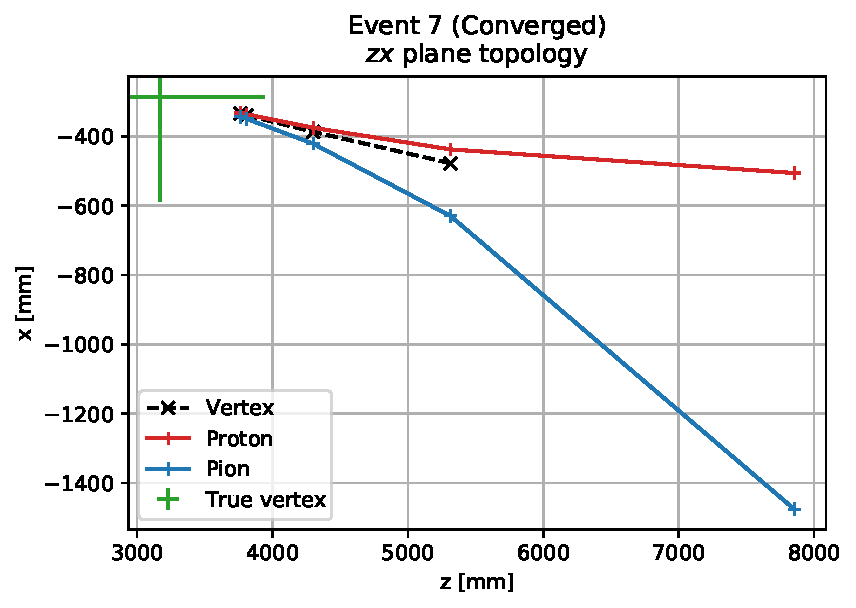
\includegraphics[width=\textwidth]{graphics/03-vertex_reconstruction/evt_converged_zx_iter.pdf}
		\caption{}
		\label{fig:zx_iter_conv}
	\end{subfigure}
	\begin{subfigure}{.45\textwidth}
		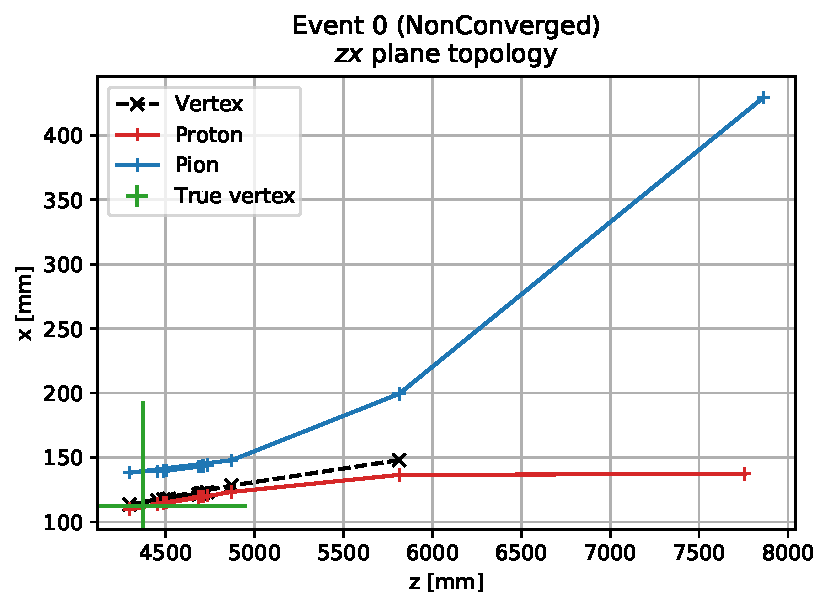
\includegraphics[width=\textwidth]{graphics/03-vertex_reconstruction/evt_failed_zx_iter.pdf}
		\caption{}
		\label{fig:zx_iter_failed}
	\end{subfigure}
	\caption[A and b.]{Dovrebbero essere gli stessi eventi della figura precedente, altrimenti non è elegante.}
	\label{fig:zx_iter_conv_vs_failed}
\end{figure}


Some more insight into the nature of this oscillation can be achieved by taking a more <<geometrical>> look, plotting inter-iteration vertex coordinates in the $zx$ plane where the LHCb magnet bends tracks according to their charge.
Figure \ref{fig:zx_iter_conv_vs_failed} compares the same events from Figure \ref{fig:z_iter_conv_vs_failed}.
Again, the converged event in Figure \ref{fig:zx_iter_conv} behaves as intended, selecting as vertex roughly the point of closest distance between the tracks (some leeway is accorded since the fit also incorporates information from $xy$ and $yz$ planes).
%% @todo: con la figura finale accertati di non stare descrivendo cazzate.
The progress in Figure \ref{fig:zx_iter_failed} is more interesting: in the failed case the estimated vertex, identified at each iteration by <<x>> markers along the dashed line, appears to gravitate \textit{around} the point of closest distance, never outright choosing it as candidate.
Significantly, the \textit{true} $\Lambda^0$ vertex (marked by the green cross) lags some \SI{50}{\centi\meter} behind it.

%% @todo: Qui metti uno di quelli brutti, però. Attualmente la distanza è troppo poca.
\begin{figure}
	\centering
	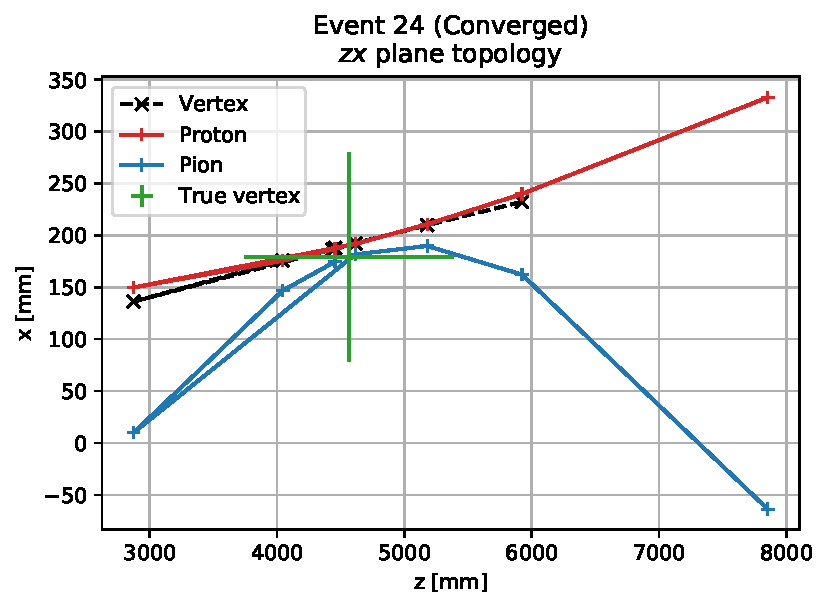
\includegraphics[width=.6\textwidth]{graphics/03-vertex_reconstruction/evt_conv_backstep_zx_iter.pdf}
	\caption{A.}
	\label{fig:zx_iter_conv_backstep}
\end{figure}

While it may be tempting to attribute the failed convergence to the comparably larger gap between proton and pion tracks at their point of closest distance, some observations are in order:
first, the deceivingly different $x$ scales in Figures \ref{fig:zx_iter_conv} and \ref{fig:zx_iter_failed} mean that in the latter tracks are closer than they may seem;
more to the point, the VF algorithm has shown to be capable of bridging an imperfect track extrapolation in converged events, as demonstrated in Figure \ref{fig:zx_iter_conv_backstep}.

\begin{figure}[t]
	\centering
	\begin{subfigure}{.45\textwidth}
		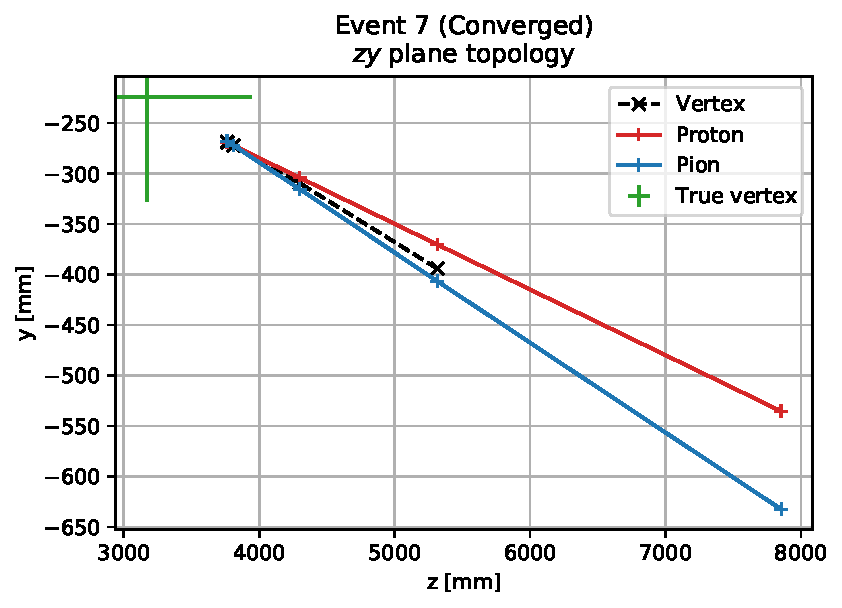
\includegraphics[width=\textwidth]{graphics/03-vertex_reconstruction/evt_converged_zy_iter.pdf}
		\caption{}
		\label{fig:zy_iter_conv}
	\end{subfigure}
	\begin{subfigure}{.45\textwidth}
		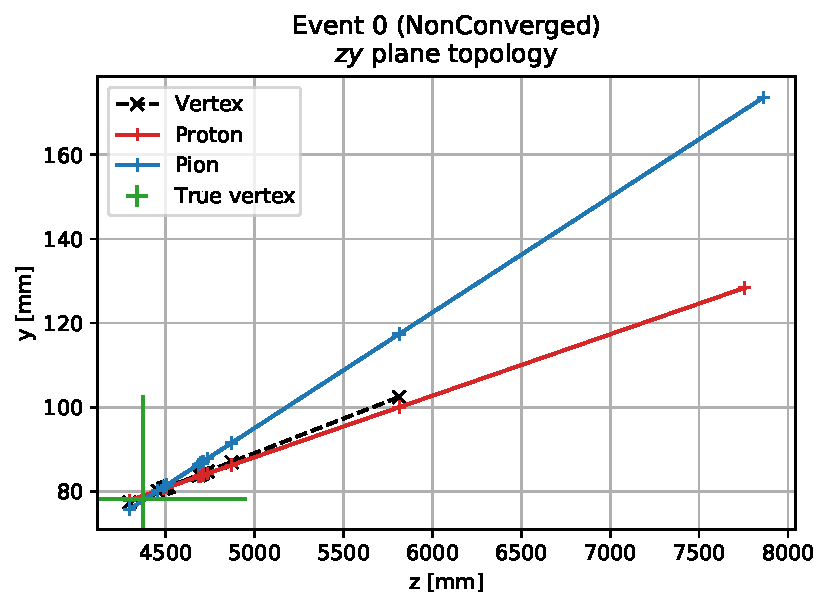
\includegraphics[width=\textwidth]{graphics/03-vertex_reconstruction/evt_failed_zy_iter.pdf}
		\caption{}
		\label{fig:zy_iter_failed}
	\end{subfigure}
	\caption[A and b.]{Devono essere gli stessi eventi della figura precedente, altrimenti non ha senso lol.}
	\label{fig:zy_iter_conv_vs_failed}
\end{figure}

We can make a more convincing remark by analyzing performance in the $yz$ plane, where tracks \textit{don't} bend.
Figure \ref{fig:zy_iter_conv} shows that, in the converged case, the $yz$ track crossing is $z$-aligned with the closest $xz$ distance point.
This doesn't happen for the failed event: while Figure \ref{fig:zy_iter_failed} shows that $yz$ tracks cross almost coinciding with the true vertex position, we have already pointed out that this is \SI{50}{cm} short of the $xz$ closest distance point.
Convergence failure for the event in Figures \ref{fig:zx_iter_failed} and \ref{fig:zy_iter_failed} can thus be interpreted through the lens of \textit{conflicting information}:
the best vertex candidate has different $z_\text{vtx}$ in the $xz$ (with magnetic field) and $yz$ (without magnetic field) planes, and the VF algorithm flip-flops between the two.

For didactic purpose, the analysis in this section has focused on just one event.
All the emerged patterns are however commonplace throughout the failed events I have examined, with the oscillating vertex behaviour in particular being a constant in almost all of them.
While every $\Lambda_b^0$ vertexing failure being the fault of $xz$ and $yz$ track mismatch would be a reckless conclusion, I have been able to use these findings, along with other from the following paragraphs, to devise a partial solution in Section \ref{sec:blowup_matrix}.

\subsection{True kinematics}
To further investigate the possible source of the oscillating behaviour outlined in Section \ref{sec:oscillation}, I have conducted a systematic comparison of kinematic features at Monte Carlo level between converged and failed events.

No difference among the two categories emerge when considering basic decay descriptors such as the momenta of all particles involved and the decay vertices of unstable particles.
Moreover, there doesn't seem to be a critical decay geometry that triggers the vertexing;
for instance, there is no evidence that $\Lambda^0 \rightarrow p\pi^-$ decays lying largely in the $xz$ plane, a setup quite unfriendly to the VF algorithm (see Section \ref{sec:lambda_endvertex_bias}), has any disproportionate representation amongst non-converged events.

\subsection{Kinematics at first measurement position}
A major discrepancy emerges when looking at particle interaction with the detector via \textit{protoparticles}.
A protoparticle is a data structure created during the LHCb event reconstruction process with the intent of encapsulating all relevant information available for the associated particle:
particle identification (PID) from the RICH and muon detectors, results from calorimeter hits and track information.
The latter contains details on momentum in relation to a certain reference point which, for stable charged particles, corresponds to the position of first measurement.

\begin{figure}[t]
	\centering
	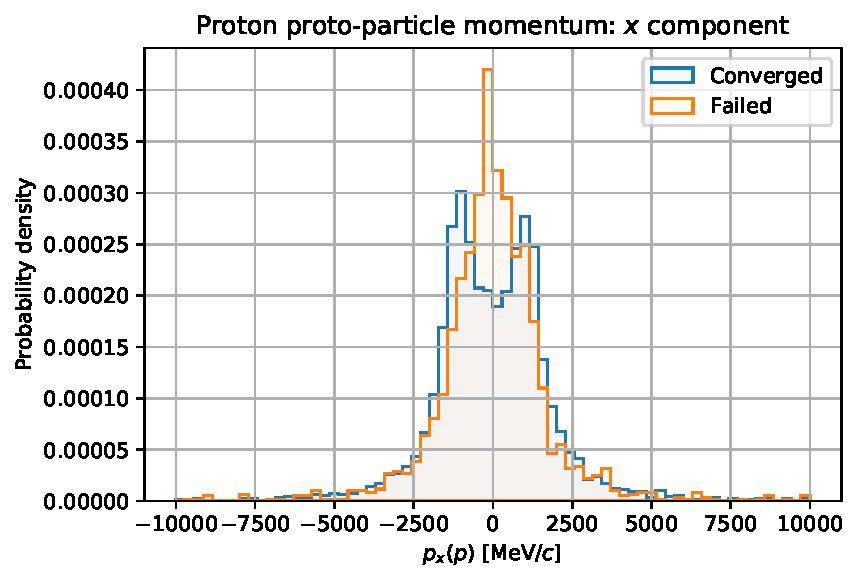
\includegraphics[width=.6\textwidth]{graphics/03-vertex_reconstruction/pp_p_momentum_x.pdf}
	\caption{A.}
	\label{fig:pp_p_px_conv_vs_failed}
\end{figure}

In the case of simulated protons from $\Lambda_b^0 \rightarrow J/\psi~\Lambda^0$ decays, the distribution of the
%true\footnote{While protoparticles result from interaction of the particle with the material, at this point I'm specifically considering the true value of the first measurement position and related momentum. Later on we'll instead delve into the \textit{reconstructed} counterparts of these quantities, which can be different as a result of poor T station measurements.}
protoparticle $p_x$ for converged and failed events shows a marked difference outlined in Figure \ref{fig:pp_p_px_conv_vs_failed}:
correctly reconstructed events tend to have a double peak roughly centered in $\approx \pm \SI{1}{\giga\electronvolt}$, while missing events have a more traditional single peak centered in $0$.

%% todo: spezza in due? Fixa anche il testo poco dopo.
\begin{figure}[t]
	\centering
	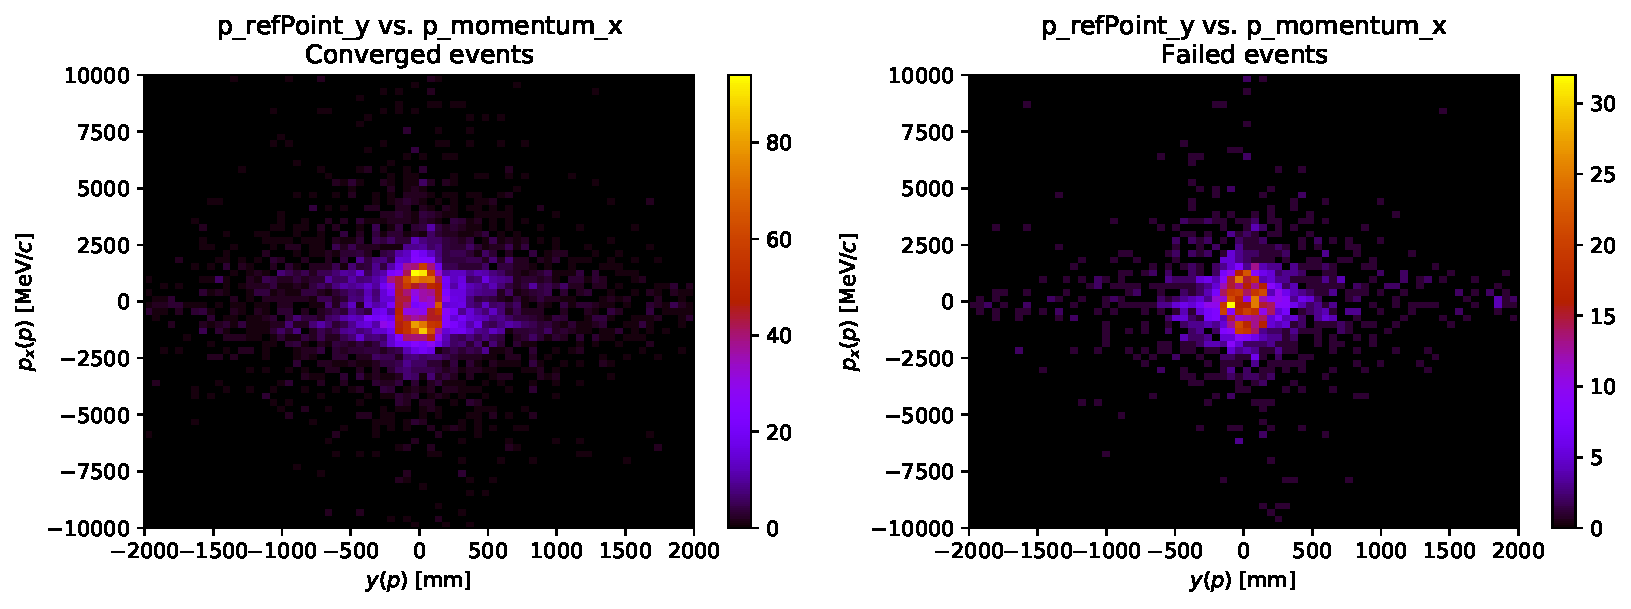
\includegraphics[width=\textwidth]{graphics/03-vertex_reconstruction/pp_p_refPoint_y_vs_p_momentum_x.pdf}
	\caption{B.}
	\label{fig:pp_p_px_vs_refpy_conv_vs_failed}
\end{figure}

Even more interestingly, this discrepancy can be put in relation to the $y$ component of the protoparticle first measurement position, as seen in Figure \ref{fig:pp_p_px_vs_refpy_conv_vs_failed}.
The ring-like structure in Figure \ref{fig:pp_p_px_vs_refpy_conv_vs_failed} implies that the vertexing process struggles to reconstruct proton protoparticles with low $p_x$ hitting the T stations at $y\approx 0$.
No such discrepancy is present in the case of pions.

A precise estimate of $p_x$ is of paramount importance for correct track measurement and extrapolation.
Even slight mistakes in angle assessment are magnified during particle transportation through long distances, especially since the T track requirement leaves no upstream constraints.
Moreover, momentum itself is computed through evaluation of the particle bending curve in the $xz$ plane induced by the magnet.
As such, it stands to reason that poor measurement of the low proton $p_x$ can have enough of an effect to throw off the vertexing algorithm.

\subsection{Kinematics at true vertex}
i.e. sottostima di pz

\begin{figure}[t]
	\centering
	\begin{subfigure}{.45\textwidth}
		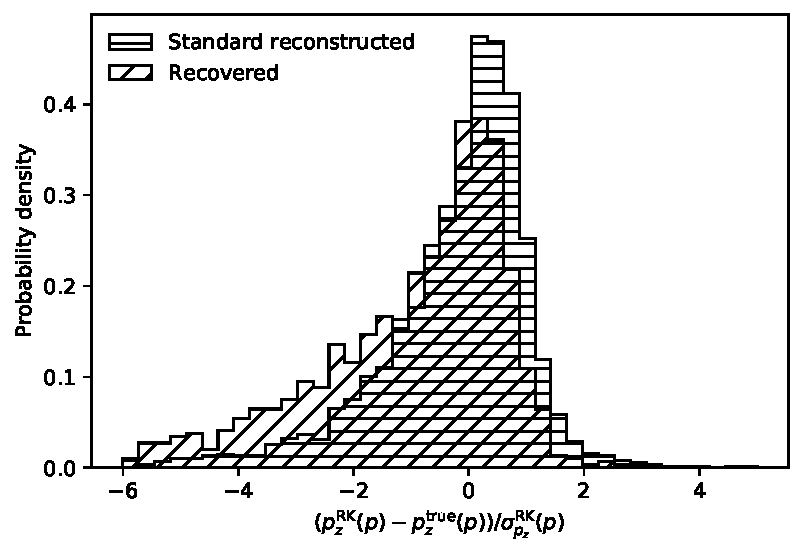
\includegraphics[width=\textwidth]{graphics/03-vertex_reconstruction/p_momentum_residual_2Dv3D_z_rel.pdf}
		\caption{}
	\end{subfigure}
	\begin{subfigure}{.45\textwidth}
		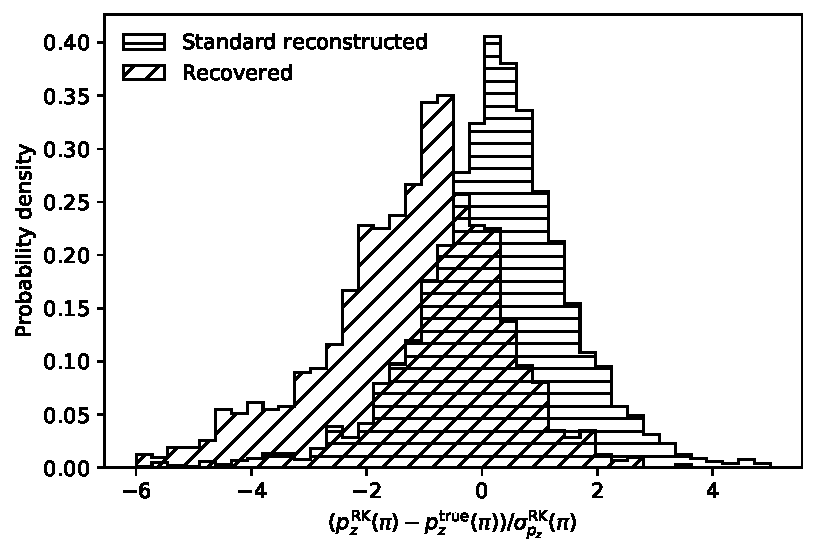
\includegraphics[width=\textwidth]{graphics/03-vertex_reconstruction/pim_momentum_residual_2Dv3D_z_rel.pdf}
		\caption{}
	\end{subfigure}
	\caption[A and b.]{Left right}
\end{figure}

\begin{figure}[t]
	\centering
	\begin{subfigure}{.45\textwidth}
		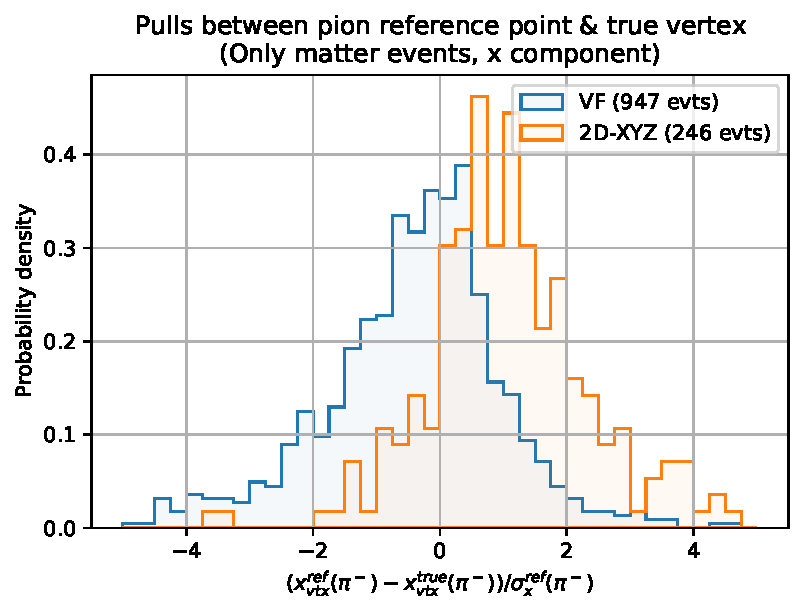
\includegraphics[width=\textwidth]{graphics/03-vertex_reconstruction/pim_refpoint_residual_2Dv3D_x_rel_matter.pdf}
		\caption{}
	\end{subfigure}
	\begin{subfigure}{.45\textwidth}
		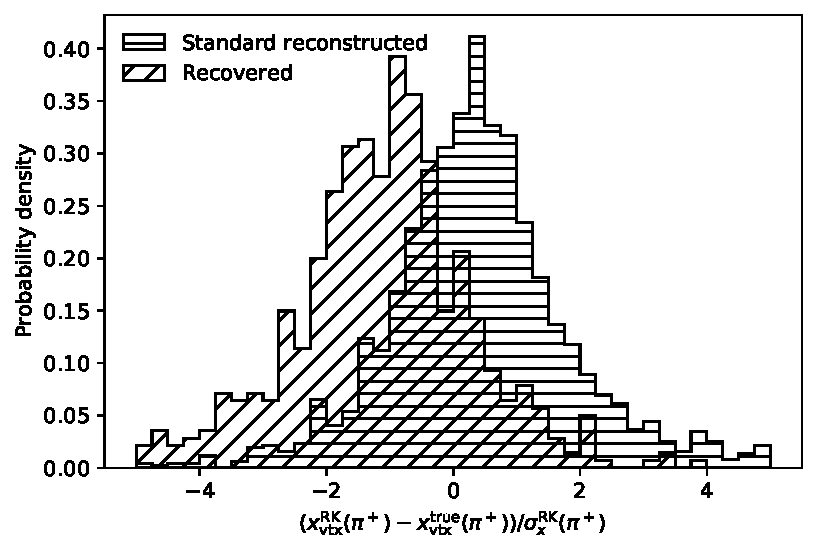
\includegraphics[width=\textwidth]{graphics/03-vertex_reconstruction/pim_refpoint_residual_2Dv3D_x_rel_antimatter.pdf}
		\caption{}
	\end{subfigure}
	\caption[A and b.]{Left right}
\end{figure}

\section{Recovery of non-converged events}
\label{sec:recovery_general}

\subsection{Recovery through interpolation}
\begin{figure}[t]
	\centering
	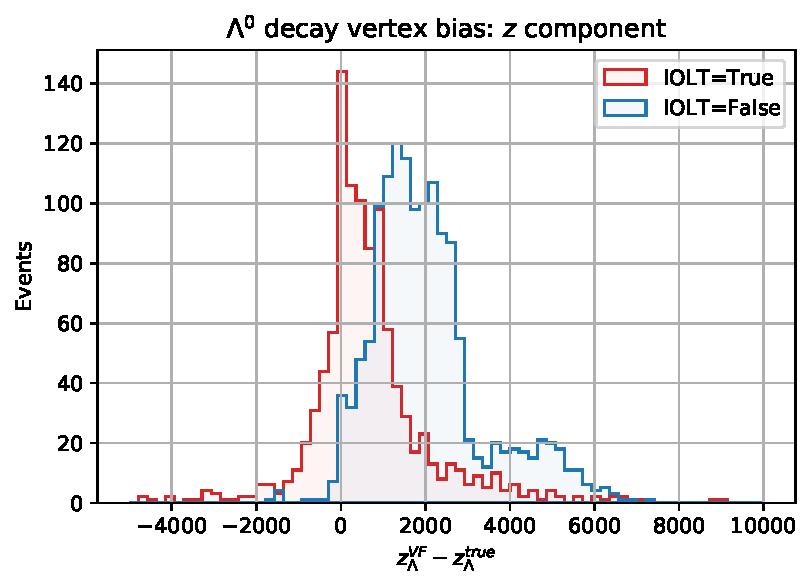
\includegraphics[width=.6\textwidth]{graphics/03-vertex_reconstruction/iolt_lambda_endvertex_z_bias.pdf}
	\caption{A.}
\end{figure}

\subsection{Recovery through refit with rescaled uncertainties}
\label{sec:blowup_matrix}

\begin{figure}[t]
	\centering
	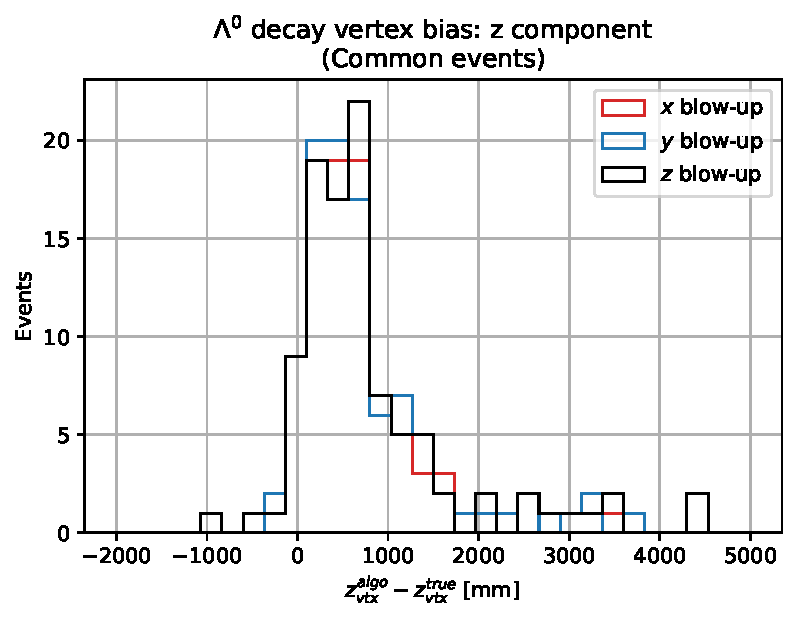
\includegraphics[width=.6\textwidth]{graphics/03-vertex_reconstruction/Lambda_endvertex_z_bias_xyz_common.pdf}
	\caption{A.}
\end{figure}

\begin{table}[t]
	\begin{center}
	\begin{tabular}{|c||c|c|c|c|}
		\hline
		Increased $\sigma$ & Recovery eff. & $\mu_\frac{1}{2}\left[\tilde{\chi}^2\right]$ & $\mu_\frac{1}{2}\left[z_\Lambda^\text{vtx} \text{ bias}\right]$ & $\mu_\frac{1}{2}\left[p_z^\text{DTF} (p) \text{ bias}\right]$ \\
		\hline
		\hline
		None (VF)  & -- & 1.0 & 429 mm & $+1.35\%$ \\
		\hline
		$\sigma_x$ & 62\% & 4.9 & 584 mm & $-0.84\%$ \\
		$\sigma_y$ & 74\% & 5.4 & 635 mm & $-0.81\%$ \\
		$\sigma_z$ & 80\% & 7.8 & 697 mm & $-1.02\%$ \\
		\hline
	\end{tabular}
	\end{center}
	\caption{Performance comparison of the three rescaled-$\sigma$ algorithms (see text for details) with a $2\%$ increase in the respective vertex position uncertainties, contrasted with the performance of the standard Vertex Fitter algorithm. Recovery efficiency is defined as the ratio of events reconstructed by a certain flavour over the total number of events recoverable by combining the three algorithms. $\mu_\frac{1}{2}$ identifies the median value. Performances for $xyz$ algorithms are computed using all events recovered by the individual flavour, including events recovered by more than one, while values for VF are computed on standard reconstructed events.}
\end{table}

\begin{figure}
	\centering
	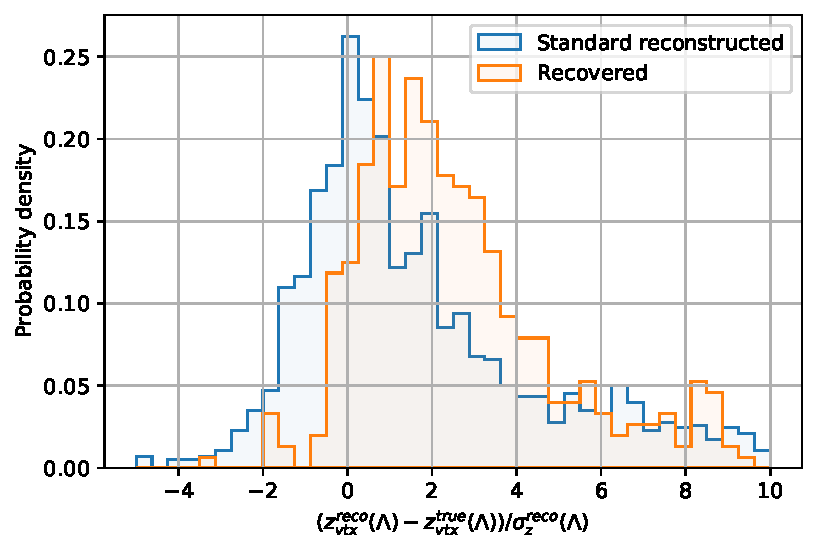
\includegraphics[width=.6\textwidth]{graphics/03-vertex_reconstruction/xyz_L_ENDVERTEX_residual_2Dv3D_z_rel.pdf}
	\caption{A.}
\end{figure}